%% CPT-Symmetric Universe -- Beamer Presentation
%% Wei-Ning Deng, Theoretical Cosmology Seminar, 17 Feb 2026
%% Compile with: pdflatex (or xelatex for better font support)

\documentclass[aspectratio=169]{beamer}

%% ---------------------------------------------------------------
%%  Packages
%% ---------------------------------------------------------------
\usepackage{amsmath,amssymb,amsfonts}
\usepackage{graphicx}
\usepackage{xcolor}
\usepackage{tikz}
\usetikzlibrary{arrows.meta, positioning, shapes.geometric}
\usepackage{hyperref}
\usepackage{booktabs}
\usepackage{multicol}

%% ---------------------------------------------------------------
%%  Theme
%% ---------------------------------------------------------------
\usetheme{default}
\usecolortheme{default}
\usefonttheme{professionalfonts}

% Clean, minimal style
\setbeamertemplate{navigation symbols}{}
\setbeamertemplate{footline}[frame number]
\setbeamertemplate{itemize items}[circle]

% Colour palette
\definecolor{cptblue}{RGB}{0,112,192}
\definecolor{cptyellow}{RGB}{255,215,0}
\definecolor{cptred}{RGB}{192,0,0}
\definecolor{cptgreen}{RGB}{0,150,60}
\definecolor{darkgray}{RGB}{50,50,50}

\setbeamercolor{frametitle}{fg=darkgray}
\setbeamercolor{title}{fg=darkgray}
\setbeamercolor{structure}{fg=cptblue}

%% ---------------------------------------------------------------
%%  Title info
%% ---------------------------------------------------------------
\title{\textbf{The CPT-Symmetric Universe:}\\
       From Quantized Curvature to K\"{a}hler-Dirac Fermions}
\author{Wei-Ning Deng \\ \small\texttt{wnd22@cam.ac.uk}}
\institute{Theoretical Cosmology Seminar}
\date{17th February 2026}

%% ---------------------------------------------------------------
%%  Helper commands
%% ---------------------------------------------------------------
\newcommand{\arxiv}[1]{[arXiv:\,#1]}
\newcommand{\Red}[1]{{\color{cptred}#1}}
\newcommand{\Blue}[1]{{\color{cptblue}#1}}
\newcommand{\Green}[1]{{\color{cptgreen}#1}}
\newcommand{\Yellow}[1]{{\color{cptyellow}#1}}

\newcommand{\figpath}{figures/}   % all figures live here

%%================================================================
\begin{document}
%%================================================================

%% ---- Title slide -----------------------------------------------
\begin{frame}[plain]
  \begin{tikzpicture}[remember picture, overlay]
    \node[at=(current page.center)] {
      \includegraphics[width=\paperwidth,height=\paperheight,
                       keepaspectratio=false]{\figpath CPT-symmetric_universe.png}
    };
    \fill[white, opacity=0.0] (current page.south west) rectangle (current page.north east);
  \end{tikzpicture}
  \vspace{-0.5cm}
  \begin{center}
    {\Large\textbf{The CPT-Symmetric Universe:}}\\[0.3em]
    {\large From Quantized Curvature to K\"{a}hler-Dirac Fermions}\\[1.8cm]
    {\normalsize Wei-Ning Deng (\texttt{wnd22@cam.ac.uk})}\\[0.2em]
    {\small Theoretical Cosmology Seminar (17th Feb 2026)}
  \end{center}
\end{frame}

%% ---- Outline ---------------------------------------------------
\begin{frame}{Outline}
  \textbf{Part 1: Introduction -- CPT-symmetric universe}\\[0.5em]
  Part 2: Theoretical Prediction of spatial curvature
  \hfill{\small (PRD.110.103528, PRD.113.023546)}\\[0.5em]
  Part 3: K\"{a}hler-Dirac Fermions -- Physical explanation for CPT
  \hfill{\small (arXiv 2511.11548)}

  \vspace{0.6cm}
  \begin{columns}[c]
    \column{0.45\textwidth}\centering
      \includegraphics[height=4cm]{\figpath wh260.jpg}\\
      {\small Will Handley (University of Cambridge)\\
       \texttt{wh260@cam.ac.uk}}
    \column{0.45\textwidth}\centering
      \includegraphics[height=4cm]{\figpath lboyle3.jpg}\\
      {\small Latham Boyle (University of Edinburgh)\\
       \texttt{Latham.Boyle@ed.ac.uk}}
  \end{columns}
\end{frame}

%%================================================================
%%  PART 1 -- Introduction: CPT-Symmetric Universe
%%================================================================
\begin{frame}{Outline}
  \textbf{\Blue{Part 1: Introduction -- CPT-symmetric universe}}\\[0.5em]
  Part 2: Theoretical Prediction of spatial curvature\\[0.5em]
  Part 3: K\"{a}hler-Dirac Fermions -- Physical explanation for CPT

  \vspace{0.6cm}
  \begin{columns}[c]
    \column{0.45\textwidth}\centering
      \includegraphics[height=4cm]{\figpath wh260.jpg}\\
      {\small Will Handley (University of Cambridge)\\
       \texttt{wh260@cam.ac.uk}}
    \column{0.45\textwidth}\centering
      \includegraphics[height=4cm]{\figpath lboyle3.jpg}\\
      {\small Latham Boyle (University of Edinburgh)\\
       \texttt{Latham.Boyle@ed.ac.uk}}
  \end{columns}
\end{frame}

%% ------------------------------------------------------------------
%%  P1-1  LCDM + SM + Cosmic Inflation
%% ------------------------------------------------------------------
\begin{frame}{$\Lambda$CDM + SM particle physics + cosmic inflation}
  \begin{center}
    \includegraphics[width=0.82\textwidth]{\figpath CMB_Timeline300_no_WMAP.jpg}
  \end{center}
\end{frame}

%% ------------------------------------------------------------------
%%  P1-2  Theoretical and Observational Challenges
%% ------------------------------------------------------------------
\begin{frame}{Theoretical and observational challenges}
  \begin{columns}[c]
    \column{0.48\textwidth}
      \begin{enumerate}
        \item \textbf{Problems in cosmology:}\\
              Cosmological constant problem, Nature of DM, etc.
        \item \textbf{Problems in particle physics:}\\
              Hierarchy problem, strong CP problem, etc.
        \item \textbf{Observational challenges:}\\
              BICEP/Keck \arxiv{2203.16556} shows tighter constraint on
              inflationary B-modes.
      \end{enumerate}
    \column{0.48\textwidth}
      \includegraphics[width=\textwidth]{\figpath r_vs_ns_bk18.pdf}
  \end{columns}
\end{frame}

%% ------------------------------------------------------------------
%%  P1-3  LCDM: 5 fundamental parameters
%% ------------------------------------------------------------------
\begin{frame}{}
  \begin{tikzpicture}[remember picture, overlay]
    \node[at=(current page.center)] {
      \includegraphics[width=\paperwidth,height=\paperheight,
                       keepaspectratio=false]{\figpath c0150405-closed_universe_artwork-spl-1.webp}
    };
  \end{tikzpicture}
  \vspace{-0.4cm}
  \begin{columns}[T]
    \column{0.52\textwidth}
      \textcolor{white}{
        \textbf{$\Lambda$CDM provides a remarkably simple\\
        description of the large-scale universe:\\
        just \Blue{5} fundamental physics parameters}\\[0.4em]
        \Blue{\textbf{the matter/energy content}}\\
        \begin{enumerate}
          \item $\rho_\Lambda$ \; cosmological constant
          \item $\rho_{DM}/\rho_B$ \; DM/baryon density
          \item $n_B/n_\gamma$ \; baryons per photon
        \end{enumerate}
        \Blue{\textbf{the large-scale geometry}}\\[0.2em]
        $\displaystyle\langle\Phi^2\rangle = \int\frac{dk}{k}\,A_\Phi
          \!\left(\frac{k}{k_*}\right)^{\!n_s-1}$
        \quad $(k_*\equiv 0.05\,\text{Mpc}^{-1})$\\[0.4em]
        \begin{enumerate}
          \setcounter{enumi}{3}
          \item $A_\Phi = (7.6\pm0.1)\times10^{-10}$ \hfill Planck CMB
          \item $n_s - 1 = -0.04\pm0.006$
        \end{enumerate}
        \vspace{0.3em}
        \footnotesize many quantities so far consistent with zero:\\
        space curvature, tensor/isocurvature perturbations, non-Gaussianity\ldots
      }
    \column{0.45\textwidth}
  \end{columns}
\end{frame}

%% ------------------------------------------------------------------
%%  P1-4  CPT-symmetric universe
%% ------------------------------------------------------------------
\begin{frame}{CPT-symmetric universe}
  \begin{center}
    \includegraphics[width=0.95\textwidth]{\figpath CPT-symmetric_universe.png}
  \end{center}
  \vspace{-0.5em}
  \begin{columns}[c]
    \column{0.5\textwidth}\centering
      $a(t)\propto t$ \quad (simple zero)
    \column{0.5\textwidth}\centering
      $\displaystyle a(t)\propto\frac{1}{t_*-t}$ \quad (simple pole)
  \end{columns}
\end{frame}

%% ------------------------------------------------------------------
%%  P1-5  CPT solves lots of problems
%% ------------------------------------------------------------------
\begin{frame}{CPT-symmetry universe can solve lots of problems}
  \small (Proposed by Latham Boyle and Neil Turok)
  \vspace{0.4em}

  \begin{center}
  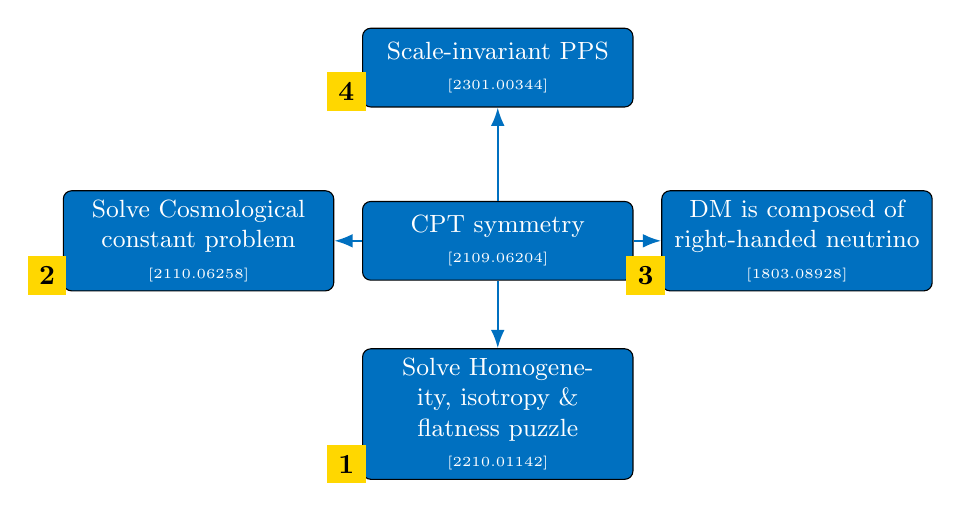
\begin{tikzpicture}[
      box/.style={draw, fill=cptblue, text=white, rounded corners=3pt,
                  text width=3.2cm, align=center, minimum height=1.0cm,
                  font=\small},
      arr/.style={-Latex, thick, cptblue},
      num/.style={fill=cptyellow, text=black, font=\bfseries,
                  inner sep=2pt, minimum size=14pt}
    ]
    \node[box] (cpt) at (0,0) {CPT symmetry \\ {\tiny [2109.06204]}};
    \node[box] (flat) at (0,-2.2) {Solve Homogeneity, isotropy \& flatness puzzle \\ {\tiny [2210.01142]}};
    \node[box] (cc)   at (-3.8,0) {Solve Cosmological constant problem \\ {\tiny [2110.06258]}};
    \node[box] (dm)   at ( 3.8,0) {DM is composed of right-handed neutrino \\ {\tiny [1803.08928]}};
    \node[box] (pps)  at (0, 2.2) {Scale-invariant PPS \\ {\tiny [2301.00344]}};

    \draw[arr] (cpt) -- (flat);
    \draw[arr] (cpt) -- (cc);
    \draw[arr] (cpt) -- (dm);
    \draw[arr] (cpt) -- (pps);

    \node[num] at ([shift={(-0.2,0.2)}]flat.south west) {1};
    \node[num] at ([shift={(-0.2,0.2)}]cc.south west)   {2};
    \node[num] at ([shift={(-0.2,0.2)}]dm.south west)   {3};
    \node[num] at ([shift={(-0.2,0.2)}]pps.south west)  {4};
  \end{tikzpicture}
  \end{center}
\end{frame}

%% ------------------------------------------------------------------
%%  P1-6  Inflation: flatness/homogeneity
%% ------------------------------------------------------------------
\begin{frame}{Homogeneity, isotropy \& flatness -- solved without inflation}
  \begin{columns}[c]
    \column{0.48\textwidth}
      \textbf{Standard approach: cosmic inflation}\\[0.5em]
      The universe expands by $\sim10^{26}$ in $\sim10^{-32}$ seconds\\[0.3em]
      \includegraphics[width=\textwidth]{\figpath Homo_iso_flat_universe.png}
    \column{0.48\textwidth}
      \textbf{CPT approach:}\\[0.3em]
      Flat, homogeneous, and isotropic universe is the \emph{most probable}.\\[0.5em]
      \footnotesize\textit{Quanta Magazine}, Nov 17, 2022;\\
      \textit{WIRED}, Jan 22, 2023
  \end{columns}
\end{frame}

%% ------------------------------------------------------------------
%%  P1-7  Black hole thermodynamics
%% ------------------------------------------------------------------
\begin{frame}{}
  \begin{tikzpicture}[remember picture, overlay]
    \node[at=(current page.center)] {
      \includegraphics[width=\paperwidth,height=\paperheight,
                       keepaspectratio=false]{\figpath BH_thermal_dynamics.png}
    };
  \end{tikzpicture}
  \begin{columns}[T]
    \column{0.6\textwidth}
      \textcolor{white}{\Large\textbf{Black hole thermodynamics}}\\[2.5cm]
      \textcolor{white}{\large Hawking temperature $T_H$,\\ gravitational entropy $S_g$}
    \column{0.38\textwidth}
      \textcolor{white}{\small Hawking \\ Bekenstein \\ Bardeen \\ Geroch \\ Gibbons \\ Hartle \\ Unruh \\ Wald}
  \end{columns}
\end{frame}

%% ------------------------------------------------------------------
%%  P1-8  Analytic solution of Friedmann equation
%% ------------------------------------------------------------------
\begin{frame}{Analytic solution of Friedmann equation in conformal time}
  \begin{columns}[c]
    \column{0.52\textwidth}
      \begin{block}{}
        \vspace{0.3em}
        \textbf{Metric:}
        \[
          ds^2 = a(t)^2\!\left(-dt^2 + \gamma_{ij}\,dx^i dx^j\right)
        \]
        \vspace{-0.5em}
        \begin{center}
          {\scriptsize scale factor \hspace{1.8cm} conformal \hspace{0.3cm} comoving symmetric\\
           \hspace{3.5cm} time \hspace{1.0cm} space (compact)}
        \end{center}
        \textbf{Friedmann equation} (Planck units):
        \[
          3\dot{a}^2 = \underbrace{r}_{\text{rad}}
                     + \underbrace{\mu a}_{\text{matter}}
                     - \underbrace{3\kappa a^2}_{\text{curvature}}
                     + \underbrace{\lambda a^4}_{\Lambda}
        \]
        \vspace{0.2em}
        \textit{General solution (Jacobi elliptic function) is periodic in imaginary time.}
        \vspace{0.3em}
      \end{block}
    \column{0.44\textwidth}
      \includegraphics[width=\textwidth]{\figpath ScaleFactorFigv2.png}
  \end{columns}
\end{frame}

%% ------------------------------------------------------------------
%%  P1-9  a(t) doubly periodic in complex plane
%% ------------------------------------------------------------------
\begin{frame}{}
  \small
  $a(t)$ is single-valued and doubly periodic in the complex $t$-plane:
  its only singularities are simple poles.
  The imaginary time period and the action computed over a period
  determine $T_H$ and the gravitational entropy $S_g$.

  \vspace{0.2em}
  \begin{columns}[c]
    \column{0.32\textwidth}\centering
      \textbf{Re}$[a(t)]$\\[0.2em]
      \includegraphics[width=\textwidth]{\figpath periodic_universe.pdf}
    \column{0.32\textwidth}\centering
      \textbf{Im}$[a(t)]$\\[0.2em]
      \includegraphics[width=\textwidth]{\figpath periodic_universe.pdf}
    \column{0.32\textwidth}\centering
      \includegraphics[width=\textwidth]{\figpath TorusFig2.png}\\
      {\scriptsize Euclidean instanton for a universe\\
       w/radiation, matter, curvature, $\Lambda$}
  \end{columns}
\end{frame}

%% ------------------------------------------------------------------
%%  P1-10  Flat universe is most probable
%% ------------------------------------------------------------------
\begin{frame}{}
  \begin{tikzpicture}[remember picture, overlay]
    \node[at=(current page.center)] {
      \includegraphics[width=\paperwidth,height=\paperheight,
                       keepaspectratio=false]{\figpath Homo_iso_flat_universe.png}
    };
  \end{tikzpicture}
  \begin{block}{}
    Flat, Homogeneous, and isotropic universe is the \textbf{most probable.}
  \end{block}
  \vspace{5.5cm}
  \centering{\small \textit{Quanta Magazine}, Nov 17, 2022; \textit{WIRED}, Jan 22, 2023}
\end{frame}

%% ------------------------------------------------------------------
%%  P1-11  Cosmological constant: cancelling anomalies
%% ------------------------------------------------------------------
\begin{frame}{}
  \begin{columns}[T]
    \column{0.55\textwidth}
      \small
      \textbf{These fields can cancel the 3 anomalies in coupling the SM to gravity}\\
      {\scriptsize L.\,Boyle + NT, arXiv:2110.06258}\\[0.5em]
      \begin{tabular}{ll}
        1. Vacuum energy & $\propto n_{s,1} - 2n_F + 2n_A + 2n_{s,0}$\\[0.3em]
        2. Conf.\ anomaly (Euler) & $\propto n_{s,1} + \tfrac{11}{2}n_F + 62n_A - 28n_{s,0}$\\[0.3em]
        3. Conf.\ anomaly (Weyl$^2$) & $\propto n_{s,1} + 3n_F + 12n_A - 8n_{s,0}$\\
      \end{tabular}\\[0.6em]
      \begin{enumerate}
        \item All three vanish iff $n_{s,1}=0$
              $\Rightarrow$ no fundamental dimension-1 scalars\\
              (the Higgs must be composite)
        \item Any two equations give $n_F = 4n_A$ and $n_{s,0} = 3n_A$
        \item For gauge group $SU(3)\times SU(2)\times U(1)$,
              predict $n_F = 48$, i.e.\ \textbf{3 fermion generations},
              each with a RH $\nu$
      \end{enumerate}
    \column{0.42\textwidth}
      \includegraphics[width=\textwidth]{\figpath SM_particles.png}\\[0.3em]
      {\small \Red{Cosmological constant problem}}
  \end{columns}
\end{frame}

%% ------------------------------------------------------------------
%%  P1-12  Extended SM: RH neutrinos + Dim-0 scalars
%% ------------------------------------------------------------------
\begin{frame}{}
  \begin{center}
    \includegraphics[height=7.5cm]{\figpath SM_particles_dim0_RHnu.png}
  \end{center}
\end{frame}

%% ------------------------------------------------------------------
%%  P1-13  Right-handed neutrinos: seesaw mechanism
%% ------------------------------------------------------------------
\begin{frame}{Right-handed neutrinos}
  \begin{center}
    \includegraphics[width=0.75\textwidth]{\figpath Seesaw_mechanism.png}
  \end{center}
  \vspace{0.3em}
  \centering
  \textit{Explain observed light neutrino masses (seesaw mechanism, 1970s)}\\[0.3em]
  Later, I'll mention a new explanation for why $\nu_R$'s \textbf{must} exist.
\end{frame}

%% ------------------------------------------------------------------
%%  P1-14  Stability of one RH neutrino
%% ------------------------------------------------------------------
\begin{frame}{Stability of one RH neutrino $\Rightarrow$ $\mathbb{Z}_2$ symm
              $\Rightarrow$ lightest $\nu$ massless}
  \begin{center}
    \includegraphics[width=0.70\textwidth]{\figpath stable_RHnu.png}
  \end{center}
  \vspace{0.3em}
  \centering
  \textit{Will be tested using EUCLID, LSST and S4}
\end{frame}

%% ------------------------------------------------------------------
%%  P1-15  RH neutrino as dark matter
%% ------------------------------------------------------------------
\begin{frame}{}
  \begin{tikzpicture}[remember picture, overlay]
    \node[at=(current page.center)] {
      \includegraphics[width=\paperwidth,height=\paperheight,
                       keepaspectratio=false]{\figpath CPT-RHnu_DM.png}
    };
  \end{tikzpicture}
\end{frame}

%% ------------------------------------------------------------------
%%  P1-16  Light neutrino observations
%% ------------------------------------------------------------------
\begin{frame}{Light neutrinos: observations}
  \begin{columns}[c]
    \column{0.50\textwidth}
      \includegraphics[width=\textwidth]{\figpath neutrino_hierachy.jpg}\\[0.3em]
      {\small
        \Green{we predict zero} for lightest neutrino mass\\[0.3em]
        Normal hierarchy: $M_\nu \equiv \sum m_\nu \approx 0.06\,\text{eV}$\\
        Inverted hierarchy: $M_\nu \approx 0.1\,\text{eV}$
      }
    \column{0.46\textwidth}
      \textbf{Current data} \hfill {\small eBOSS 2007.08991}\\[0.3em]
      \includegraphics[width=\textwidth]{\figpath mnu_constraints.pdf}
  \end{columns}
\end{frame}

%% ------------------------------------------------------------------
%%  P1-17  Extended SM with RH neutrinos + Dim-0 scalars (detail)
%% ------------------------------------------------------------------
\begin{frame}{Extended Standard Model}
  \begin{center}
    \includegraphics[height=7.2cm]{\figpath SM_particles_dim0_RHnu.png}
  \end{center}
\end{frame}

%% ------------------------------------------------------------------
%%  P1-18  Dim-0 scalar field seeds scale-invariant PPS
%% ------------------------------------------------------------------
\begin{frame}{Dim-0 scalar field seeds scale-invariant PPS}
  \begin{columns}[c]
    \column{0.55\textwidth}
      \begin{align*}
        S &= -\tfrac{1}{2}\int d^4x\sqrt{-g}\;\varphi\Delta_4\varphi \\[0.5em]
        \langle\delta\varphi_i(\eta,\mathbf{x})\,\delta\varphi_j(\eta,\mathbf{x}')\rangle
        &= \delta_{ij}\int\frac{d^3\mathbf{k}}{(2\pi)^3}\,
           \frac{e^{i\mathbf{k}\cdot(\mathbf{x}-\mathbf{x}')}}{4ak^3}\\[0.5em]
        \mathcal{P}_\mathcal{R}
        &= \frac{3^2 5^3}{7(2\pi)^4}
           \left(\frac{c_\beta^{SM}}{\mathcal{N}_{eff}}\right)^{\!2}
      \end{align*}
      \vspace{0.5em}
      \textbf{Predicted:} $A = 12.9\pm4.5\times10^{-10}$,
      $n_s \approx 1 - 7\alpha_3(M_P)/\pi = 0.958$\\[0.3em]
      \textbf{Observed (Planck):} $A = 21\pm0.3\times10^{-10}$, $n_s = 0.9587\pm0.0056$
    \column{0.42\textwidth}
      \includegraphics[width=\textwidth]{\figpath Quantum_Fluctuations.gif}
  \end{columns}
\end{frame}

%% ------------------------------------------------------------------
%%  P1-19  CPT solves lots of problems (transition slide)
%% ------------------------------------------------------------------
\begin{frame}{CPT-symmetry universe can solve lots of problems}
  \small (Proposed by Latham Boyle and Neil Turok)
  \vspace{0.4em}

  \begin{center}
  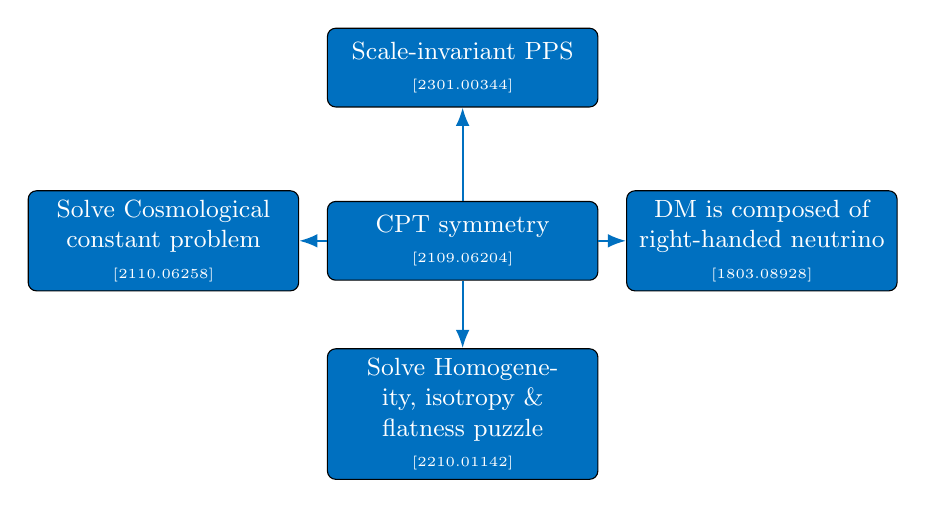
\begin{tikzpicture}[
      box/.style={draw, fill=cptblue, text=white, rounded corners=3pt,
                  text width=3.2cm, align=center, minimum height=1.0cm,
                  font=\small},
      arr/.style={-Latex, thick, cptblue}
    ]
    \node[box] (cpt) at (0,0) {CPT symmetry \\ {\tiny [2109.06204]}};
    \node[box] (flat) at (0,-2.2) {Solve Homogeneity, isotropy \& flatness puzzle \\ {\tiny [2210.01142]}};
    \node[box] (cc)   at (-3.8,0) {Solve Cosmological constant problem \\ {\tiny [2110.06258]}};
    \node[box] (dm)   at ( 3.8,0) {DM is composed of right-handed neutrino \\ {\tiny [1803.08928]}};
    \node[box] (pps)  at (0, 2.2) {Scale-invariant PPS \\ {\tiny [2301.00344]}};

    \draw[arr] (cpt) -- (flat);
    \draw[arr] (cpt) -- (cc);
    \draw[arr] (cpt) -- (dm);
    \draw[arr] (cpt) -- (pps);
  \end{tikzpicture}

  \vspace{0.3em}
  \Red{\textbf{How about perturbations?}}
  \end{center}
\end{frame}

%%================================================================
%%  PART 2 -- Theoretical Prediction of Spatial Curvature
%%================================================================
\begin{frame}{Outline}
  Part 1: Introduction -- CPT-symmetric universe\\[0.5em]
  \textbf{\Blue{Part 2: Theoretical Prediction of spatial curvature}}\\[0.5em]
  Part 3: K\"{a}hler-Dirac Fermions -- Physical explanation for CPT

  \vspace{0.6cm}
  \begin{columns}[c]
    \column{0.45\textwidth}\centering
      \includegraphics[height=4cm]{\figpath wh260.jpg}\\
      {\small Will Handley (University of Cambridge)\\
       \texttt{wh260@cam.ac.uk}}
    \column{0.45\textwidth}\centering
      \includegraphics[height=4cm]{\figpath lboyle3.jpg}\\
      {\small Latham Boyle (University of Edinburgh)\\
       \texttt{Latham.Boyle@ed.ac.uk}}
  \end{columns}
\end{frame}

%% ------------------------------------------------------------------
%%  P2-1  Evolution of Perturbations
%% ------------------------------------------------------------------
\begin{frame}{Evolution of Perturbations}
  \hfill{\small Lasenby et al.\ \arxiv{2104.02521}}

  \vspace{0.1em}
  $\Phi(k,\eta) \propto \cos\theta(k,\eta)$
  \quad\quad
  $\Phi$: Newtonian potential,\;
  $V$: velocity perturbation of radiation,\;
  $\delta$: density perturbation of radiation

  \vspace{0.2em}
  \begin{columns}[c]
    \column{0.48\textwidth}
      \includegraphics[width=\textwidth]{\figpath perturbation_solutions_transMatrix_timeseries_s-a.pdf}
    \column{0.48\textwidth}
      \includegraphics[width=\textwidth]{\figpath perturbation_solutions_transMatrix_timeseries_s-a.pdf}
  \end{columns}

  \vspace{0.2em}
  \begin{block}{}
    \centering
    $\theta(k,\eta=\eta_\infty) = m\dfrac{\pi}{2},\quad m\in\mathbb{N}$
    \hspace{1em}
    \Red{\textbf{Perturbations also have to be symmetric!}}
  \end{block}
\end{frame}

%% ------------------------------------------------------------------
%%  P2-2  Perturbations should be CPT-symmetric
%% ------------------------------------------------------------------
\begin{frame}{Perturbations should also be CPT-symmetric}
  \begin{center}
    \includegraphics[width=0.88\textwidth]{\figpath posi_neg_energy_waves.png}
  \end{center}
\end{frame}

%% ------------------------------------------------------------------
%%  P2-3  Discrete allowed k: standing waves
%% ------------------------------------------------------------------
\begin{frame}{}
  \begin{columns}[c]
    \column{0.35\textwidth}
      \includegraphics[width=\textwidth]{\figpath standing_waves.png}\\[0.3em]
      {\small 1/4 wave, 3/4 waves, 5/4 waves, 7/4 waves}
    \column{0.60\textwidth}
      \centering
      $\theta(k,\eta=\eta_\infty)$ should be $m\dfrac{\pi}{2},\; m\in\mathbb{N}$\\[0.3em]
      \includegraphics[width=0.85\textwidth]{\figpath dtheta_dk_OmegaK.png}
  \end{columns}
\end{frame}

%% ------------------------------------------------------------------
%%  P2-4  Spatial boundary condition in closed universe
%% ------------------------------------------------------------------
\begin{frame}{Spatial boundary condition in closed universe}
  \begin{columns}[c]
    \column{0.52\textwidth}
      Closed universes have finite space
      $\Rightarrow$ an additional spatial boundary condition
      (in spherical harmonics)\\[0.5em]
      $\Rightarrow$ wave vectors have to be integers:
      \[
        k = n \in [1,2,3,\ldots]
      \]
      \vspace{0.3em}
      \Red{Matching the two discrete $k$ sets\\
           $\Rightarrow$ \textbf{constrains the curvature value.}}
    \column{0.44\textwidth}
      \includegraphics[width=\textwidth]{\figpath c0150405-closed_universe_artwork-spl-1.webp}
  \end{columns}
\end{frame}

%% ------------------------------------------------------------------
%%  P2-5  End of universe eta_inf depends on curvature
%% ------------------------------------------------------------------
\begin{frame}{The end of the universe $\eta_\infty$ depends on curvature}
  \begin{columns}[c]
    \column{0.48\textwidth}
      Larger curvature $\rightarrow$ larger $\eta_\infty$\\[0.5em]
      Since $\Delta k \propto 1/\eta_\infty$, larger $\eta_\infty$
      means smaller $\Delta k$.\\[0.5em]
      {\small (larger curvature: $\Omega_{\kappa,0}$ more negative)}
    \column{0.48\textwidth}
      \includegraphics[width=\textwidth]{\figpath loga-OmegaK.png}
  \end{columns}
\end{frame}

%% ------------------------------------------------------------------
%%  P2-6  Idea: adjust curvature so discrete k become integers
%% ------------------------------------------------------------------
\begin{frame}{Idea}
  \begin{columns}[c]
    \column{0.48\textwidth}
      Larger curvature has steeper $\theta(k,\eta=\eta_\infty)$
      $\rightarrow$ has discrete $k$ with smaller spacing $\Delta k$.\\[0.5em]
      \Red{\textbf{Idea:} Adjusting the curvature values, such that
           the discrete $k$ become integers.}
    \column{0.48\textwidth}
      \includegraphics[width=\textwidth]{\figpath Theta_diff_OmegaK.png}
  \end{columns}
\end{frame}

%% ------------------------------------------------------------------
%%  P2-7  Gradient condition
%% ------------------------------------------------------------------
\begin{frame}{}
  \begin{columns}[c]
    \column{0.40\textwidth}
      \begin{block}{}
        The gradient $\dfrac{2}{\pi}\dfrac{d\theta}{dk}$
        should be $N$ or $1/N$
      \end{block}
    \column{0.56\textwidth}
      \includegraphics[width=\textwidth]{\figpath dtheta_dk_OmegaK.png}\\
      {\small Current curvature $\Omega_\kappa = -0.000$}
  \end{columns}
\end{frame}

%% ------------------------------------------------------------------
%%  P2-8  Result: gradient vs curvature
%% ------------------------------------------------------------------
\begin{frame}{Result}
  \begin{columns}[c]
    \column{0.40\textwidth}
      \begin{enumerate}
        \item The gradient increases while increasing curvature.
        \item It goes to infinity at $\Omega_{\kappa,0}\simeq -0.012$;
              curvature larger than this would cause a big crunch.
      \end{enumerate}
    \column{0.56\textwidth}
      \includegraphics[width=\textwidth]{\figpath K_crit.pdf}
  \end{columns}
\end{frame}

%% ------------------------------------------------------------------
%%  P2-9  Consider real cosmology
%% ------------------------------------------------------------------
\begin{frame}{Consider Real Cosmology}
  \begin{enumerate}
    \item Solve Friedmann equation containing matter:
          \[
            3\dot{a}^2 = \lambda\!\left(a^4 - 3\tilde{\kappa}a^2
                          + \tilde{m}a + \tilde{r}\right)
          \]
    \item Transform to cosmological parameters:
          \[
            \Omega_m = \tilde{m}\Omega_\Lambda/a_0^3,\quad
            \Omega_K = -3\tilde{\kappa}\Omega_\Lambda/a_0^2,\quad
            \Omega_r = \tilde{r}\Omega_\Lambda/a_0^4
          \]
    \item Solve perturbation equations numerically (containing higher-order
          Boltzmann terms) to get allowed wave vectors.
  \end{enumerate}
\end{frame}

%% ------------------------------------------------------------------
%%  P2-10  (Anti-)symmetric perturbation solutions
%% ------------------------------------------------------------------
\begin{frame}{(Anti-)symmetric Perturbation solutions}
  \begin{center}
    \includegraphics[width=0.92\textwidth]{\figpath perturbation_solutions_transMatrix_timeseries_s-a.pdf}
  \end{center}
\end{frame}

%% ------------------------------------------------------------------
%%  P2-11  Contour plot of Delta k
%% ------------------------------------------------------------------
\begin{frame}{}
  \begin{columns}[c]
    \column{0.40\textwidth}
      \[
        c(\Omega_K,\Omega_m,\Omega_b,h) = N \in \mathbb{N}
      \]
    \column{0.56\textwidth}
      \includegraphics[width=\textwidth]{\figpath DeltaK_contourPlot.png}
  \end{columns}
\end{frame}

%% ------------------------------------------------------------------
%%  P2-12  Compare with CMB
%% ------------------------------------------------------------------
\begin{frame}{Compare with CMB}
  \begin{columns}[c]
    \column{0.46\textwidth}
      Modify Boltzmann code CLASS to see how sparse wave vectors
      affect CMB power spectrum.
      \begin{enumerate}
        \item More fluctuations if $N$ and curvature ($\tilde{\kappa}$) become large.
        \item However, since $\Delta\tilde{k} = N\sqrt{\tilde{\kappa}}$,
              $N$ and $\tilde{\kappa}$ are negatively correlated
              $\rightarrow$ never both large.
        \item The fluctuation behaviour could be ignored.
      \end{enumerate}
    \column{0.50\textwidth}
      \includegraphics[width=\textwidth]{\figpath CMB_diff_nuspacing.pdf}
  \end{columns}
\end{frame}

%% ------------------------------------------------------------------
%%  P2-13  CMB constraint: triangle plot
%% ------------------------------------------------------------------
\begin{frame}{CMB constraint}
  \begin{columns}[c]
    \column{0.38\textwidth}
      Filter Planck MCMC data with the $\Delta k\in\mathbb{N}$ constraint.\\[0.5em]
      Need joint analysis to break the degeneracy.
    \column{0.58\textwidth}
      \includegraphics[width=\textwidth]{\figpath Planck_TrianglePlot_diffDeltaK.pdf}
  \end{columns}
\end{frame}

%% ------------------------------------------------------------------
%%  P2-14  Chi-squared vs Omega_K
%% ------------------------------------------------------------------
\begin{frame}{}
  \begin{center}
    \includegraphics[width=0.72\textwidth]{\figpath Planck_omegak_vs_chi2.pdf}
  \end{center}
\end{frame}

%% ------------------------------------------------------------------
%%  P2-15  How about low-k modes?
%% ------------------------------------------------------------------
\begin{frame}{How about low-$k$ modes?}
  \begin{columns}[c]
    \column{0.52\textwidth}
      \begin{enumerate}
        \item So far we only consider large $k$ modes, where allowed wave
              vectors become equally spaced.
        \item The valid solutions should satisfy both spatial and temporal BC
              $\rightarrow$ could be constructed by linear combination of both bases:
              \[
                \Phi(x,t) = \sum_{n=1}^\infty c_n\phi_n
                           = \sum_{m=1}^\infty \tilde{c}_m\tilde{\phi}_m
              \]
        \item The linear combination coefficients are eigenvectors of
              mixing matrix $M$ with eigenvalue $= 1$.
      \end{enumerate}
    \column{0.44\textwidth}
      \includegraphics[width=\textwidth]{\figpath mapping_valid_sol.png}
  \end{columns}
\end{frame}

%% ------------------------------------------------------------------
%%  P2-16  Result: linear combined solutions on cylinder
%% ------------------------------------------------------------------
\begin{frame}{Result}
  \begin{columns}[c]
    \column{0.40\textwidth}
      \includegraphics[width=\textwidth]{\figpath eigenvalue_2d_N25_Nt500_T3.14_m1.50_cylinder1.pdf}
    \column{0.56\textwidth}
      \includegraphics[width=\textwidth]{\figpath linear_combined_sols.png}
  \end{columns}
\end{frame}

%%================================================================
%%  PART 3 -- Kähler-Dirac Fermions
%%================================================================
\begin{frame}{Outline}
  Part 1: Introduction -- CPT-symmetric universe\\[0.5em]
  Part 2: Theoretical Prediction of spatial curvature\\[0.5em]
  \textbf{\Blue{Part 3: K\"{a}hler-Dirac Fermions -- Physical explanation for CPT}}

  \vspace{0.6cm}
  \begin{columns}[c]
    \column{0.45\textwidth}\centering
      \includegraphics[height=4cm]{\figpath wh260.jpg}\\
      {\small Will Handley (University of Cambridge)\\
       \texttt{wh260@cam.ac.uk}}
    \column{0.45\textwidth}\centering
      \includegraphics[height=4cm]{\figpath lboyle3.jpg}\\
      {\small Latham Boyle (University of Edinburgh)\\
       \texttt{Latham.Boyle@ed.ac.uk}}
  \end{columns}
\end{frame}

%% ------------------------------------------------------------------
%%  P3-1  Problem: fermion doubling on the lattice
%% ------------------------------------------------------------------
\begin{frame}{Fermion doubling problem on the lattice}
  \begin{columns}[c]
    \column{0.52\textwidth}
      \textbf{Wilson's lattice gauge theory} works beautifully for bosons:
      \begin{itemize}
        \item 0-forms (scalars) $\to$ vertices
        \item 1-forms (gauge fields) $\to$ links
        \item 2-forms (field strengths) $\to$ plaquettes
      \end{itemize}
      \vspace{0.5em}
      \textbf{Problem with spinors:} no natural $p$-form interpretation
      $\Rightarrow$ placed on vertices $\Rightarrow$ \Red{extra doublers in the continuum limit}\\[0.4em]
      Chiral theory $\xrightarrow{\text{lattice}}$ non-chiral theory
      \hfill {\small (Nielsen--Ninomiya, 1981)}
    \column{0.44\textwidth}
      \includegraphics[width=\textwidth]{\figpath lattice.png}
  \end{columns}
\end{frame}

%% ------------------------------------------------------------------
%%  P3-2  Kähler-Dirac fermions
%% ------------------------------------------------------------------
\begin{frame}{K\"{a}hler-Dirac (KD) fermions}
  \textbf{Key idea:} KD fermions are $p$-forms -- they live naturally on any cell complex.

  \vspace{0.5em}
  \textbf{KD field} $\Phi$ is a \emph{polyform}: sum of $p$-forms ($p=0,\ldots,4$) with $16$ complex components.

  \vspace{0.4em}
  \textbf{KD action and equation:}
  \[
    S_{KD} = \langle\bar\Phi|(K-m)\Phi\rangle, \qquad
    (d - d^\dagger - m)\Phi = 0
  \]
  where $K = d - d^\dagger$,\quad $-K^2 = \square$ (wave operator on forms).

  \vspace{0.4em}
  Replacing $dx^\mu \to \gamma^\mu$ assembles the 16 components into a $4\times4$ matrix $\Psi$:
  \[
    (i\gamma^\mu\partial_\mu - m)\Psi = 0
    \quad\Rightarrow\quad
    S_{KD} = \int d^4x\;\mathrm{Tr}\!\left[\bar\Psi(i\slashed\partial - m)\Psi\right]
  \]
  with $\bar\Psi \equiv \gamma^0\Psi^\dagger\gamma^0$ (extra $\gamma^0$ on the left!).

  \vspace{0.3em}
  \Blue{Bonus:} restricted KD fermions $\to$ Pati-Salam multiplets $\to$ explains SM structure \hfill{\small [Catterall et al.]}
\end{frame}

%% ------------------------------------------------------------------
%%  P3-3  The wrong-sign problem
%% ------------------------------------------------------------------
\begin{frame}{The wrong-sign problem in Lorentzian signature}
  Diagonalise the extra $\gamma^0$: $\gamma^0 = \Omega\Lambda\Omega^T$,
  $\Lambda = \mathrm{diag}(+1,+1,-1,-1)$.\\[0.5em]
  In terms of $\Psi' \equiv \Psi\Omega$:
  \[
    S_{KD} = \int d^4x\;\mathrm{Tr}\!\left[\Lambda\,\Psi'{}^\dagger\gamma^0
             (i\slashed\partial - m)\Psi'\right]
  \]
  \begin{itemize}
    \item Columns 1--2 of $\Psi'$: \Green{right sign} $\Rightarrow$ positive norm
    \item Columns 3--4 of $\Psi'$: \Red{wrong sign} $\Rightarrow$ \Red{negative norm states (ghosts)!}
  \end{itemize}

  \vspace{0.5em}
  \textbf{Resolution} (Donoghue \& Menezes): a wrong-sign action = reversal of causality arrow
  $=$ \Blue{$PT$ reversal}.

  \vspace{0.4em}
  $\Rightarrow$ the two pairs of columns live on \textbf{two sheets} of spacetime, related by $PT$ symmetry
  (or, equivalently, $i \leftrightarrow -i$).
\end{frame}

%% ------------------------------------------------------------------
%%  P3-4  Two-sheeted spacetime
%% ------------------------------------------------------------------
\begin{frame}{Two-sheeted spacetime}
  \begin{columns}[c]
    \column{0.50\textwidth}
      \begin{itemize}
        \item \Blue{Forward sheet} ($\Lambda_{ii}=+1$, cols 1--2):
              standard quantum mechanics with $e^{iS}$, $[x,p]=+i$
        \item \Blue{Backward sheet} ($\Lambda_{ii}=-1$, cols 3--4):
              uses $e^{-iS}$, $[x,p]=-i$
        \item The two sheets are \textbf{$PT$ mirrors} of each other
        \item Positive energy, positive norm on \emph{both} sheets
      \end{itemize}
      \vspace{0.5em}
      \textit{``Our" Big Bang is the junction of the two sheets --\\
      exactly the CPT-symmetric universe picture!}
    \column{0.46\textwidth}
      \includegraphics[width=\textwidth]{\figpath CPT-symmetric_universe.png}
  \end{columns}
\end{frame}

%% ------------------------------------------------------------------
%%  P3-5  KD-Majorana condition
%% ------------------------------------------------------------------
\begin{frame}{KD-Majorana condition}
  \textbf{Problem:} Two independent non-interacting sheets would double the particle content.

  \vspace{0.4em}
  \textbf{Solution:} Impose the \Blue{KD-Majorana condition}
  \[
    \Psi^c \equiv (i\gamma^2)\Psi^*(i\gamma^2) = \Psi
  \]
  In terms of $\Psi'$, the four columns are forced to take the form:
  \[
    \Psi' = \bigl(\psi_1,\;\psi_2,\;-\psi_2^c,\;\psi_1^c\bigr)
  \]

  \vspace{0.3em}
  \begin{columns}[c]
    \column{0.55\textwidth}
      \begin{itemize}
        \item A LH particle on the forward sheet is \emph{always} paired with
              a RH anti-particle on the backward sheet
        \item \Blue{Physical meaning:} CPT symmetry -- every particle has
              a mirror (anti-)partner on the other sheet
        \item No unphysical doubling of the SM
      \end{itemize}
    \column{0.42\textwidth}
      \includegraphics[width=\textwidth]{\figpath KD_Majorana.png}
  \end{columns}
\end{frame}

%% ------------------------------------------------------------------
%%  P3-6  Relation to the Standard Model
%% ------------------------------------------------------------------
\begin{frame}{Relation to the Standard Model}
  One SM generation (including $\nu_R$) = 16 Weyl spinors
  $=$ 4 KD-Majorana fields.\\[0.4em]
  Following Pati-Salam: allocate to four copies $\Psi'_{A=0,1,2,3}$
  \[
    \Psi'_0 = \chi_0 + \chi_0^c,\quad
    \chi_0 = \begin{pmatrix}\nu_L & e_L \\ \nu_R & e_R\end{pmatrix}
    \quad\text{(leptons)}
  \]
  \[
    \Psi'_i = \chi_i + \chi_i^c,\quad
    \chi_i = \begin{pmatrix}u_L^i & d_L^i \\ u_R^i & d_R^i\end{pmatrix}
    \quad\text{(quarks, color }i=1,2,3)
  \]

  \vspace{0.3em}
  \textbf{Fermion kinetic terms unify:}
  \[
    \mathcal{L}_\text{KD} = \mathrm{Tr}\!\left[\bar\Psi_A(i\slashed\partial)\Psi_A\right],\quad A=0,\ldots,3
  \]
  Gauging $SU(3)\subset SU(4)$ and $SU(2)\times U(1)\subset U(2,2)$
  reproduces \emph{all} SM fermion kinetic terms.
\end{frame}

%% ------------------------------------------------------------------
%%  P3-7  Yukawa couplings unify
%% ------------------------------------------------------------------
\begin{frame}{Yukawa couplings unify in KD formalism}
  Standard Yukawa Lagrangian (4 separate terms):
  \[
    \tilde h^T\bar q_L u_R y_u + h^T\bar q_L d_R y_d
    + \tilde h^T\bar\ell_L \nu_R y_\nu + h^T\bar\ell_L e_R y_e
    + \text{h.c.}
  \]

  \vspace{0.3em}
  \textbf{KD formulation} (single compact expression):
  \[
    \mathcal{L}_Y = \mathrm{Tr}\!\left[
      \mathcal{H}^T\,\widehat\Psi_{A,L}^{\prime\,i}\,\Psi_{A,R}^{\prime\,j}\,
      \mathcal{Y}_A^{ij}
    \right] + \text{h.c.}
  \]
  where $\mathcal{H}$ is the \emph{KD Higgs field} and
  $\mathcal{Y}_A^{ij}$ the \emph{KD Yukawa matrix}.

  \vspace{0.4em}
  \begin{itemize}
    \item Expanding for leptons reproduces exactly the two lepton Yukawa terms
    \item Forward sheet $\leftrightarrow$ particles; backward sheet $\leftrightarrow$ antiparticles
    \item \Blue{All four SM Yukawa sectors unified in one line}
  \end{itemize}
\end{frame}

%% ------------------------------------------------------------------
%%  P3-8  Why must RH neutrinos exist? (KD explanation)
%% ------------------------------------------------------------------
\begin{frame}{Why must $\nu_R$'s exist? -- a new explanation}
  \begin{columns}[c]
    \column{0.55\textwidth}
      \textbf{Old explanation:} seesaw mechanism explains small
      $\nu_L$ masses.\\[0.5em]
      \textbf{New (KD) explanation:}
      \begin{itemize}
        \item Each KD-Majorana field contains both LH \emph{and} RH components
        \item Including $\nu_L$ in $\Psi'_0$ \emph{forces} the existence of $\nu_R$
              on the same sheet
        \item $\nu_R$ is \textbf{required by the geometry} of the KD field --
              not just by phenomenology
      \end{itemize}
      \vspace{0.5em}
      \Green{This is the new explanation promised at the start of the talk!}
    \column{0.42\textwidth}
      \includegraphics[width=\textwidth]{\figpath Seesaw_mechanism.png}
  \end{columns}
\end{frame}

%% ------------------------------------------------------------------
%%  P3-9  Connection to CPT-symmetric universe
%% ------------------------------------------------------------------
\begin{frame}{Connection to the CPT-symmetric universe}
  \begin{columns}[c]
    \column{0.52\textwidth}
      \textbf{Question:} \textit{Why} does the Big Bang act as a CPT mirror?\\[0.5em]
      The CPT-symmetric universe was motivated by observations
      (reflecting boundary conditions on perturbations at early times).\\[0.4em]
      \textbf{KD answer:} The KD-Majorana condition \emph{requires} every particle
      to have a mirror (anti-)partner on the other sheet.\\[0.4em]
      \Blue{The Big Bang is precisely the junction where the two spacetime sheets meet.}
      \vspace{0.3em}
      \[
        \underbrace{\text{KD-Majorana}}_{\text{field theory}}
        \;\longleftrightarrow\;
        \underbrace{\text{CPT mirror at bang}}_{\text{cosmology}}
      \]
    \column{0.44\textwidth}
      \includegraphics[width=\textwidth]{\figpath CPT-symmetric_universe.png}
  \end{columns}
\end{frame}

%% ------------------------------------------------------------------
%%  P3-10  Black mirror
%% ------------------------------------------------------------------
\begin{frame}{Black mirror: an alternative to black holes}
  \begin{columns}[c]
    \column{0.50\textwidth}
      \textbf{Standard picture:} black hole has an interior.\\[0.4em]
      \textbf{Black mirror proposal} \hfill{\small [Tzanavaris et al.]}
      \begin{itemize}
        \item The interior \emph{does not exist}
        \item The horizon is a mirror connecting our exterior to
              the ``other'' exterior (anti-universe)
        \item Each infalling particle from our universe
              \emph{annihilates} with its anti-partner from
              the anti-universe at the horizon
      \end{itemize}
      \vspace{0.3em}
      \Green{The KD-Majorana condition explains why infalling
      particles are paired in this way.}
    \column{0.46\textwidth}
      \includegraphics[width=\textwidth]{\figpath Penrose_diagram_BHMirror.png}\\[0.3em]
      \includegraphics[width=\textwidth]{\figpath annihilate_BHmirror.png}
  \end{columns}
\end{frame}

%% ------------------------------------------------------------------
%%  P3-11  Periodic black mirror
%% ------------------------------------------------------------------
\begin{frame}{Periodic black mirror}
  \begin{center}
    \includegraphics[width=0.80\textwidth]{\figpath Periodic_BHMirror.png}
  \end{center}
  \vspace{0.2em}
  \centering
  {\small A periodic array of black mirrors -- consistent with the doubly-periodic
  structure of $a(t)$ in the complex plane.}
\end{frame}

%% ------------------------------------------------------------------
%%  P3-12  Summary
%% ------------------------------------------------------------------
\begin{frame}{Summary}
  \begin{columns}[T]
    \column{0.48\textwidth}
      \textbf{Part 1: Introduction}
      \begin{itemize}\small
        \item CPT-symmetric universe solves flatness, CC problem,
              DM, scale-invariant PPS
        \item Extended SM: 3 RH neutrinos + 36 Dim-0 scalars
        \item Lightest $\nu$ massless; $\nu_R$ as DM ($M\approx5\times10^8$ GeV)
      \end{itemize}
      \vspace{0.5em}
      \textbf{Part 2: Quantized curvature}
      \begin{itemize}\small
        \item CPT symmetry $\Rightarrow$ perturbations must be symmetric
        \item Matching temporal \& spatial BCs $\Rightarrow$ discrete $k$
        \item Predicts $\Omega_K < 0$, constrained by Planck MCMC
      \end{itemize}
    \column{0.48\textwidth}
      \textbf{Part 3: K\"{a}hler-Dirac fermions} \hfill{\small arXiv:2511.11548}
      \begin{itemize}\small
        \item KD fermions = polyforms; live naturally on lattice
        \item Wrong-sign columns $\Rightarrow$ two-sheeted spacetime
        \item KD-Majorana condition: every particle paired with
              mirror anti-partner on other sheet
        \item Unifies all SM fermion kinetic \& Yukawa terms
        \item \Blue{Explains \emph{why} the Big Bang is a CPT mirror}
        \item Application: black mirror (alternative to BH interior)
      \end{itemize}
      \vspace{0.4em}
      \centering
      \textbf{\Blue{Thank you!}}\\
      \small\texttt{wnd22@cam.ac.uk}
  \end{columns}
\end{frame}

%%================================================================
\end{document}
